\chapter{Background}\label{chap:background}
This chapter explores various works done by the industry and researchers which acts as the basis for the later topics in the dissertation. 

\section{The Microservice Architecture}
Usually, a set of small autonomous services which can be deployed in various ways, being advantageous for continuous delivery pipelines.  This allows the application which adopts the architecture to scale much easier on hardware which is suitable for the services. 

As the architecture is made up on smaller services, they are highly maintainable, testable and more fault tolerant, i.e if one service were to go down, the rest of the system does not, and this would allow for faster recovery times.  


\section{The Microservice Architecture}
Usually, a set of small loosely coupled components that can be deployed, scaled and tested independently which make up for a cloud-native application, more commonly known as the Microservice architecture. A major reason for the introduction of this architecture has been the ever-increasing demand for deploying cloud-native applications as various industries embrace a software-driven model. 

Using the microservice architecture comes with its own set of unique features, these features allow for new deployment patterns to be discussed and why this paper exists. 

Such features are listed below: 

\begin{itemize}
    \item Highly maintainable and testable 
    \item Loosely coupled with other services 
    \item Independently deployable 
    \item Capable of being deployed by a smaller team
\end{itemize}

\textbf{Why are microservice often used in industry now and what advantages do these have?}

\section{Deployment Patterns}
\textbf{WHY DO THESE PATTERNS MATTER?? }
% https://www.nginx.com/blog/deploying-microservices/
Microservice applications consist of multiple services, which are created using different technologies. Each service has specific run-time requirements, such as needing appropriate CPU, Memory and I/O resources, or requiring a certain number of instances for the service to keep up with demand. This means that deploying a microservice application can be challenging as the services should be able to deploy in a speedy, reliably and be cost-effective manner. 

The following patterns are set out to remedy issues with deploying services to the cloud, these can be used interchangeably if required. The patterns itself have been set out by the author of microservices.io, Chris Richardson \cite{Chr19}. 

\subsection{Pattern 1: Single Service Instances per Host}
    \begin{figure}[H]
        \centering
        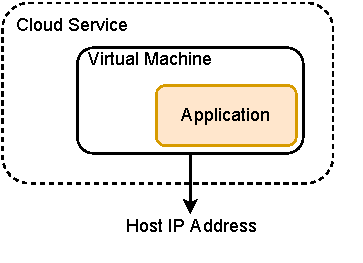
\includegraphics[width=0.45\linewidth]{images/Pattern-1.pdf}
        \caption{An example "application" is used for visualizing the pattern mentioned here.}
    \end{figure}  

In this pattern of deploying a microserivce application, multiple service instances or the entire application is provisioned on a single physical or virtual host in a cloud service. This is also often the easiest and most traditional pattern which can also work well with other architectures \citep{Chr19}. The application once deployed runs on a well known port, such as port 8080, which allows for HTTPS traffic to be directed towards the host, using the hosts IP address \citep{Chr19}. 

There can be various benefits and drawbacks for using this pattern.  Firstly, similar services can be deployed and are able to run more efficiently as the services share the same operating system and server resources  \textbf{reducing communication time between services as they no longer have to communicate over the internet.} Since all the services or a set of services are deployed on the same machines, they do not need to wait for other services in the application to start up, and can be easily deployed again or restarted. 

Whilst the benefits makes it an appealing pattern to use, there are also some drawback's, as multiple services run on the same host, there is minimal isolation between the services, making it harder to accurately track resource utilization per service, and a misbehaving services could consume a major chunk of the resource availability. 

\textit{Another known issue occurs since multiple services are to be deployed on the same server, each service needs to be documented well and have it's own configuration file for dependencies, if these are not well maintained, the complexity of figuring out which service is missing dependencies increase's complexity at the deployment stage.  }



\subsection{Pattern 2 : Multiple Service Instance per Multiple Hosts}
    \begin{figure}[H]
        \centering
        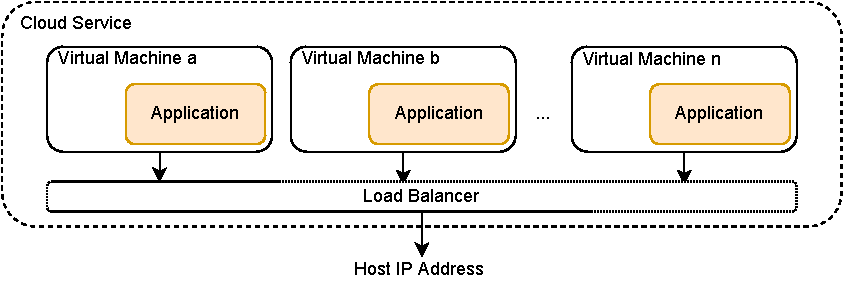
\includegraphics[width=0.9\linewidth]{images/Pattern-2.pdf}
        \caption{An example application is used for visualizing the pattern mentioned here.}
    \end{figure}  

This pattern is quite similar to Pattern 1, with the key difference being where multiple machine are provisioned to run multiple instances of the services.   


\subsection{Pattern 3 : Single service instance per multiple hosts}
    \begin{figure}[H]
        \centering
        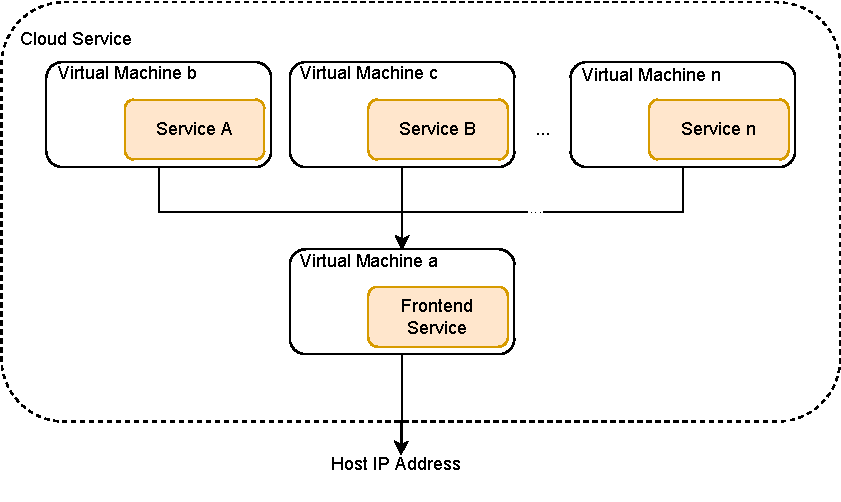
\includegraphics[width=0.8\linewidth]{images/Pattern-3.pdf}
        \caption{An example application is used for visualizing the pattern mentioned here.}
    \end{figure}  



\section{Infrastructure As A Platform -Terraform}
% https://amazicworld.com/building-auto-scaling-groupss-in-azure-with-terraform/

The Infrastructure as code platform used for the project is an open source tool developed by HashiCorp called Terraform, it uses a declarative language to deploy and manage infrastructure across a variety of cloud providers, private clouds and virtualization platforms. 


\subsection{Terraform Azure}
\begin{lstlisting}
    terraform {
      required_providers {
        azurerm = {
          source = "hashicorp/azurerm"
          version = "~>2.0"
        }
      }
    }
    
    # Use a pre-created resource group
    data "azurerm_resource_group" "{resource_name}" {
    	name = "{resource_name}"
    }
    
\end{lstlisting}

\subsection{Modules}
Modules are used to create light weight abstractions which can be used to describe infrastructure in terms of the architecture instead of fixed variable names. 
\subsubsection{Root Module}
\subsubsection{Child Modules}
